\documentclass[11pt]{article}

    \usepackage[breakable]{tcolorbox}
    \usepackage{parskip} % Stop auto-indenting (to mimic markdown behaviour)
    
    \usepackage{iftex}
    \ifPDFTeX
    	\usepackage[T1]{fontenc}
    	\usepackage{mathpazo}
    \else
    	\usepackage{fontspec}
    \fi

    % Basic figure setup, for now with no caption control since it's done
    % automatically by Pandoc (which extracts ![](path) syntax from Markdown).
    \usepackage{graphicx}
    % Maintain compatibility with old templates. Remove in nbconvert 6.0
    \let\Oldincludegraphics\includegraphics
    % Ensure that by default, figures have no caption (until we provide a
    % proper Figure object with a Caption API and a way to capture that
    % in the conversion process - todo).
    \usepackage{caption}
    \DeclareCaptionFormat{nocaption}{}
    \captionsetup{format=nocaption,aboveskip=0pt,belowskip=0pt}

    \usepackage{float}
    \floatplacement{figure}{H} % forces figures to be placed at the correct location
    \usepackage{xcolor} % Allow colors to be defined
    \usepackage{enumerate} % Needed for markdown enumerations to work
    \usepackage{geometry} % Used to adjust the document margins
    \usepackage{amsmath} % Equations
    \usepackage{amssymb} % Equations
    \usepackage{textcomp} % defines textquotesingle
    % Hack from http://tex.stackexchange.com/a/47451/13684:
    \AtBeginDocument{%
        \def\PYZsq{\textquotesingle}% Upright quotes in Pygmentized code
    }
    \usepackage{upquote} % Upright quotes for verbatim code
    \usepackage{eurosym} % defines \euro
    \usepackage[mathletters]{ucs} % Extended unicode (utf-8) support
    \usepackage{fancyvrb} % verbatim replacement that allows latex
    \usepackage{grffile} % extends the file name processing of package graphics 
                         % to support a larger range
    \makeatletter % fix for old versions of grffile with XeLaTeX
    \@ifpackagelater{grffile}{2019/11/01}
    {
      % Do nothing on new versions
    }
    {
      \def\Gread@@xetex#1{%
        \IfFileExists{"\Gin@base".bb}%
        {\Gread@eps{\Gin@base.bb}}%
        {\Gread@@xetex@aux#1}%
      }
    }
    \makeatother
    \usepackage[Export]{adjustbox} % Used to constrain images to a maximum size
    \adjustboxset{max size={0.9\linewidth}{0.9\paperheight}}

    % The hyperref package gives us a pdf with properly built
    % internal navigation ('pdf bookmarks' for the table of contents,
    % internal cross-reference links, web links for URLs, etc.)
    \usepackage{hyperref}
    % The default LaTeX title has an obnoxious amount of whitespace. By default,
    % titling removes some of it. It also provides customization options.
    \usepackage{titling}
    \usepackage{longtable} % longtable support required by pandoc >1.10
    \usepackage{booktabs}  % table support for pandoc > 1.12.2
    \usepackage[inline]{enumitem} % IRkernel/repr support (it uses the enumerate* environment)
    \usepackage[normalem]{ulem} % ulem is needed to support strikethroughs (\sout)
                                % normalem makes italics be italics, not underlines
    \usepackage{mathrsfs}
    

    
    % Colors for the hyperref package
    \definecolor{urlcolor}{rgb}{0,.145,.698}
    \definecolor{linkcolor}{rgb}{.71,0.21,0.01}
    \definecolor{citecolor}{rgb}{.12,.54,.11}

    % ANSI colors
    \definecolor{ansi-black}{HTML}{3E424D}
    \definecolor{ansi-black-intense}{HTML}{282C36}
    \definecolor{ansi-red}{HTML}{E75C58}
    \definecolor{ansi-red-intense}{HTML}{B22B31}
    \definecolor{ansi-green}{HTML}{00A250}
    \definecolor{ansi-green-intense}{HTML}{007427}
    \definecolor{ansi-yellow}{HTML}{DDB62B}
    \definecolor{ansi-yellow-intense}{HTML}{B27D12}
    \definecolor{ansi-blue}{HTML}{208FFB}
    \definecolor{ansi-blue-intense}{HTML}{0065CA}
    \definecolor{ansi-magenta}{HTML}{D160C4}
    \definecolor{ansi-magenta-intense}{HTML}{A03196}
    \definecolor{ansi-cyan}{HTML}{60C6C8}
    \definecolor{ansi-cyan-intense}{HTML}{258F8F}
    \definecolor{ansi-white}{HTML}{C5C1B4}
    \definecolor{ansi-white-intense}{HTML}{A1A6B2}
    \definecolor{ansi-default-inverse-fg}{HTML}{FFFFFF}
    \definecolor{ansi-default-inverse-bg}{HTML}{000000}

    % common color for the border for error outputs.
    \definecolor{outerrorbackground}{HTML}{FFDFDF}

    % commands and environments needed by pandoc snippets
    % extracted from the output of `pandoc -s`
    \providecommand{\tightlist}{%
      \setlength{\itemsep}{0pt}\setlength{\parskip}{0pt}}
    \DefineVerbatimEnvironment{Highlighting}{Verbatim}{commandchars=\\\{\}}
    % Add ',fontsize=\small' for more characters per line
    \newenvironment{Shaded}{}{}
    \newcommand{\KeywordTok}[1]{\textcolor[rgb]{0.00,0.44,0.13}{\textbf{{#1}}}}
    \newcommand{\DataTypeTok}[1]{\textcolor[rgb]{0.56,0.13,0.00}{{#1}}}
    \newcommand{\DecValTok}[1]{\textcolor[rgb]{0.25,0.63,0.44}{{#1}}}
    \newcommand{\BaseNTok}[1]{\textcolor[rgb]{0.25,0.63,0.44}{{#1}}}
    \newcommand{\FloatTok}[1]{\textcolor[rgb]{0.25,0.63,0.44}{{#1}}}
    \newcommand{\CharTok}[1]{\textcolor[rgb]{0.25,0.44,0.63}{{#1}}}
    \newcommand{\StringTok}[1]{\textcolor[rgb]{0.25,0.44,0.63}{{#1}}}
    \newcommand{\CommentTok}[1]{\textcolor[rgb]{0.38,0.63,0.69}{\textit{{#1}}}}
    \newcommand{\OtherTok}[1]{\textcolor[rgb]{0.00,0.44,0.13}{{#1}}}
    \newcommand{\AlertTok}[1]{\textcolor[rgb]{1.00,0.00,0.00}{\textbf{{#1}}}}
    \newcommand{\FunctionTok}[1]{\textcolor[rgb]{0.02,0.16,0.49}{{#1}}}
    \newcommand{\RegionMarkerTok}[1]{{#1}}
    \newcommand{\ErrorTok}[1]{\textcolor[rgb]{1.00,0.00,0.00}{\textbf{{#1}}}}
    \newcommand{\NormalTok}[1]{{#1}}
    
    % Additional commands for more recent versions of Pandoc
    \newcommand{\ConstantTok}[1]{\textcolor[rgb]{0.53,0.00,0.00}{{#1}}}
    \newcommand{\SpecialCharTok}[1]{\textcolor[rgb]{0.25,0.44,0.63}{{#1}}}
    \newcommand{\VerbatimStringTok}[1]{\textcolor[rgb]{0.25,0.44,0.63}{{#1}}}
    \newcommand{\SpecialStringTok}[1]{\textcolor[rgb]{0.73,0.40,0.53}{{#1}}}
    \newcommand{\ImportTok}[1]{{#1}}
    \newcommand{\DocumentationTok}[1]{\textcolor[rgb]{0.73,0.13,0.13}{\textit{{#1}}}}
    \newcommand{\AnnotationTok}[1]{\textcolor[rgb]{0.38,0.63,0.69}{\textbf{\textit{{#1}}}}}
    \newcommand{\CommentVarTok}[1]{\textcolor[rgb]{0.38,0.63,0.69}{\textbf{\textit{{#1}}}}}
    \newcommand{\VariableTok}[1]{\textcolor[rgb]{0.10,0.09,0.49}{{#1}}}
    \newcommand{\ControlFlowTok}[1]{\textcolor[rgb]{0.00,0.44,0.13}{\textbf{{#1}}}}
    \newcommand{\OperatorTok}[1]{\textcolor[rgb]{0.40,0.40,0.40}{{#1}}}
    \newcommand{\BuiltInTok}[1]{{#1}}
    \newcommand{\ExtensionTok}[1]{{#1}}
    \newcommand{\PreprocessorTok}[1]{\textcolor[rgb]{0.74,0.48,0.00}{{#1}}}
    \newcommand{\AttributeTok}[1]{\textcolor[rgb]{0.49,0.56,0.16}{{#1}}}
    \newcommand{\InformationTok}[1]{\textcolor[rgb]{0.38,0.63,0.69}{\textbf{\textit{{#1}}}}}
    \newcommand{\WarningTok}[1]{\textcolor[rgb]{0.38,0.63,0.69}{\textbf{\textit{{#1}}}}}
    
    
    % Define a nice break command that doesn't care if a line doesn't already
    % exist.
    \def\br{\hspace*{\fill} \\* }
    % Math Jax compatibility definitions
    \def\gt{>}
    \def\lt{<}
    \let\Oldtex\TeX
    \let\Oldlatex\LaTeX
    \renewcommand{\TeX}{\textrm{\Oldtex}}
    \renewcommand{\LaTeX}{\textrm{\Oldlatex}}
    % Document parameters
    % Document title
    \title{chapter-1-0}
    
    
    
    
    
% Pygments definitions
\makeatletter
\def\PY@reset{\let\PY@it=\relax \let\PY@bf=\relax%
    \let\PY@ul=\relax \let\PY@tc=\relax%
    \let\PY@bc=\relax \let\PY@ff=\relax}
\def\PY@tok#1{\csname PY@tok@#1\endcsname}
\def\PY@toks#1+{\ifx\relax#1\empty\else%
    \PY@tok{#1}\expandafter\PY@toks\fi}
\def\PY@do#1{\PY@bc{\PY@tc{\PY@ul{%
    \PY@it{\PY@bf{\PY@ff{#1}}}}}}}
\def\PY#1#2{\PY@reset\PY@toks#1+\relax+\PY@do{#2}}

\@namedef{PY@tok@w}{\def\PY@tc##1{\textcolor[rgb]{0.73,0.73,0.73}{##1}}}
\@namedef{PY@tok@c}{\let\PY@it=\textit\def\PY@tc##1{\textcolor[rgb]{0.25,0.50,0.50}{##1}}}
\@namedef{PY@tok@cp}{\def\PY@tc##1{\textcolor[rgb]{0.74,0.48,0.00}{##1}}}
\@namedef{PY@tok@k}{\let\PY@bf=\textbf\def\PY@tc##1{\textcolor[rgb]{0.00,0.50,0.00}{##1}}}
\@namedef{PY@tok@kp}{\def\PY@tc##1{\textcolor[rgb]{0.00,0.50,0.00}{##1}}}
\@namedef{PY@tok@kt}{\def\PY@tc##1{\textcolor[rgb]{0.69,0.00,0.25}{##1}}}
\@namedef{PY@tok@o}{\def\PY@tc##1{\textcolor[rgb]{0.40,0.40,0.40}{##1}}}
\@namedef{PY@tok@ow}{\let\PY@bf=\textbf\def\PY@tc##1{\textcolor[rgb]{0.67,0.13,1.00}{##1}}}
\@namedef{PY@tok@nb}{\def\PY@tc##1{\textcolor[rgb]{0.00,0.50,0.00}{##1}}}
\@namedef{PY@tok@nf}{\def\PY@tc##1{\textcolor[rgb]{0.00,0.00,1.00}{##1}}}
\@namedef{PY@tok@nc}{\let\PY@bf=\textbf\def\PY@tc##1{\textcolor[rgb]{0.00,0.00,1.00}{##1}}}
\@namedef{PY@tok@nn}{\let\PY@bf=\textbf\def\PY@tc##1{\textcolor[rgb]{0.00,0.00,1.00}{##1}}}
\@namedef{PY@tok@ne}{\let\PY@bf=\textbf\def\PY@tc##1{\textcolor[rgb]{0.82,0.25,0.23}{##1}}}
\@namedef{PY@tok@nv}{\def\PY@tc##1{\textcolor[rgb]{0.10,0.09,0.49}{##1}}}
\@namedef{PY@tok@no}{\def\PY@tc##1{\textcolor[rgb]{0.53,0.00,0.00}{##1}}}
\@namedef{PY@tok@nl}{\def\PY@tc##1{\textcolor[rgb]{0.63,0.63,0.00}{##1}}}
\@namedef{PY@tok@ni}{\let\PY@bf=\textbf\def\PY@tc##1{\textcolor[rgb]{0.60,0.60,0.60}{##1}}}
\@namedef{PY@tok@na}{\def\PY@tc##1{\textcolor[rgb]{0.49,0.56,0.16}{##1}}}
\@namedef{PY@tok@nt}{\let\PY@bf=\textbf\def\PY@tc##1{\textcolor[rgb]{0.00,0.50,0.00}{##1}}}
\@namedef{PY@tok@nd}{\def\PY@tc##1{\textcolor[rgb]{0.67,0.13,1.00}{##1}}}
\@namedef{PY@tok@s}{\def\PY@tc##1{\textcolor[rgb]{0.73,0.13,0.13}{##1}}}
\@namedef{PY@tok@sd}{\let\PY@it=\textit\def\PY@tc##1{\textcolor[rgb]{0.73,0.13,0.13}{##1}}}
\@namedef{PY@tok@si}{\let\PY@bf=\textbf\def\PY@tc##1{\textcolor[rgb]{0.73,0.40,0.53}{##1}}}
\@namedef{PY@tok@se}{\let\PY@bf=\textbf\def\PY@tc##1{\textcolor[rgb]{0.73,0.40,0.13}{##1}}}
\@namedef{PY@tok@sr}{\def\PY@tc##1{\textcolor[rgb]{0.73,0.40,0.53}{##1}}}
\@namedef{PY@tok@ss}{\def\PY@tc##1{\textcolor[rgb]{0.10,0.09,0.49}{##1}}}
\@namedef{PY@tok@sx}{\def\PY@tc##1{\textcolor[rgb]{0.00,0.50,0.00}{##1}}}
\@namedef{PY@tok@m}{\def\PY@tc##1{\textcolor[rgb]{0.40,0.40,0.40}{##1}}}
\@namedef{PY@tok@gh}{\let\PY@bf=\textbf\def\PY@tc##1{\textcolor[rgb]{0.00,0.00,0.50}{##1}}}
\@namedef{PY@tok@gu}{\let\PY@bf=\textbf\def\PY@tc##1{\textcolor[rgb]{0.50,0.00,0.50}{##1}}}
\@namedef{PY@tok@gd}{\def\PY@tc##1{\textcolor[rgb]{0.63,0.00,0.00}{##1}}}
\@namedef{PY@tok@gi}{\def\PY@tc##1{\textcolor[rgb]{0.00,0.63,0.00}{##1}}}
\@namedef{PY@tok@gr}{\def\PY@tc##1{\textcolor[rgb]{1.00,0.00,0.00}{##1}}}
\@namedef{PY@tok@ge}{\let\PY@it=\textit}
\@namedef{PY@tok@gs}{\let\PY@bf=\textbf}
\@namedef{PY@tok@gp}{\let\PY@bf=\textbf\def\PY@tc##1{\textcolor[rgb]{0.00,0.00,0.50}{##1}}}
\@namedef{PY@tok@go}{\def\PY@tc##1{\textcolor[rgb]{0.53,0.53,0.53}{##1}}}
\@namedef{PY@tok@gt}{\def\PY@tc##1{\textcolor[rgb]{0.00,0.27,0.87}{##1}}}
\@namedef{PY@tok@err}{\def\PY@bc##1{{\setlength{\fboxsep}{\string -\fboxrule}\fcolorbox[rgb]{1.00,0.00,0.00}{1,1,1}{\strut ##1}}}}
\@namedef{PY@tok@kc}{\let\PY@bf=\textbf\def\PY@tc##1{\textcolor[rgb]{0.00,0.50,0.00}{##1}}}
\@namedef{PY@tok@kd}{\let\PY@bf=\textbf\def\PY@tc##1{\textcolor[rgb]{0.00,0.50,0.00}{##1}}}
\@namedef{PY@tok@kn}{\let\PY@bf=\textbf\def\PY@tc##1{\textcolor[rgb]{0.00,0.50,0.00}{##1}}}
\@namedef{PY@tok@kr}{\let\PY@bf=\textbf\def\PY@tc##1{\textcolor[rgb]{0.00,0.50,0.00}{##1}}}
\@namedef{PY@tok@bp}{\def\PY@tc##1{\textcolor[rgb]{0.00,0.50,0.00}{##1}}}
\@namedef{PY@tok@fm}{\def\PY@tc##1{\textcolor[rgb]{0.00,0.00,1.00}{##1}}}
\@namedef{PY@tok@vc}{\def\PY@tc##1{\textcolor[rgb]{0.10,0.09,0.49}{##1}}}
\@namedef{PY@tok@vg}{\def\PY@tc##1{\textcolor[rgb]{0.10,0.09,0.49}{##1}}}
\@namedef{PY@tok@vi}{\def\PY@tc##1{\textcolor[rgb]{0.10,0.09,0.49}{##1}}}
\@namedef{PY@tok@vm}{\def\PY@tc##1{\textcolor[rgb]{0.10,0.09,0.49}{##1}}}
\@namedef{PY@tok@sa}{\def\PY@tc##1{\textcolor[rgb]{0.73,0.13,0.13}{##1}}}
\@namedef{PY@tok@sb}{\def\PY@tc##1{\textcolor[rgb]{0.73,0.13,0.13}{##1}}}
\@namedef{PY@tok@sc}{\def\PY@tc##1{\textcolor[rgb]{0.73,0.13,0.13}{##1}}}
\@namedef{PY@tok@dl}{\def\PY@tc##1{\textcolor[rgb]{0.73,0.13,0.13}{##1}}}
\@namedef{PY@tok@s2}{\def\PY@tc##1{\textcolor[rgb]{0.73,0.13,0.13}{##1}}}
\@namedef{PY@tok@sh}{\def\PY@tc##1{\textcolor[rgb]{0.73,0.13,0.13}{##1}}}
\@namedef{PY@tok@s1}{\def\PY@tc##1{\textcolor[rgb]{0.73,0.13,0.13}{##1}}}
\@namedef{PY@tok@mb}{\def\PY@tc##1{\textcolor[rgb]{0.40,0.40,0.40}{##1}}}
\@namedef{PY@tok@mf}{\def\PY@tc##1{\textcolor[rgb]{0.40,0.40,0.40}{##1}}}
\@namedef{PY@tok@mh}{\def\PY@tc##1{\textcolor[rgb]{0.40,0.40,0.40}{##1}}}
\@namedef{PY@tok@mi}{\def\PY@tc##1{\textcolor[rgb]{0.40,0.40,0.40}{##1}}}
\@namedef{PY@tok@il}{\def\PY@tc##1{\textcolor[rgb]{0.40,0.40,0.40}{##1}}}
\@namedef{PY@tok@mo}{\def\PY@tc##1{\textcolor[rgb]{0.40,0.40,0.40}{##1}}}
\@namedef{PY@tok@ch}{\let\PY@it=\textit\def\PY@tc##1{\textcolor[rgb]{0.25,0.50,0.50}{##1}}}
\@namedef{PY@tok@cm}{\let\PY@it=\textit\def\PY@tc##1{\textcolor[rgb]{0.25,0.50,0.50}{##1}}}
\@namedef{PY@tok@cpf}{\let\PY@it=\textit\def\PY@tc##1{\textcolor[rgb]{0.25,0.50,0.50}{##1}}}
\@namedef{PY@tok@c1}{\let\PY@it=\textit\def\PY@tc##1{\textcolor[rgb]{0.25,0.50,0.50}{##1}}}
\@namedef{PY@tok@cs}{\let\PY@it=\textit\def\PY@tc##1{\textcolor[rgb]{0.25,0.50,0.50}{##1}}}

\def\PYZbs{\char`\\}
\def\PYZus{\char`\_}
\def\PYZob{\char`\{}
\def\PYZcb{\char`\}}
\def\PYZca{\char`\^}
\def\PYZam{\char`\&}
\def\PYZlt{\char`\<}
\def\PYZgt{\char`\>}
\def\PYZsh{\char`\#}
\def\PYZpc{\char`\%}
\def\PYZdl{\char`\$}
\def\PYZhy{\char`\-}
\def\PYZsq{\char`\'}
\def\PYZdq{\char`\"}
\def\PYZti{\char`\~}
% for compatibility with earlier versions
\def\PYZat{@}
\def\PYZlb{[}
\def\PYZrb{]}
\makeatother


    % For linebreaks inside Verbatim environment from package fancyvrb. 
    \makeatletter
        \newbox\Wrappedcontinuationbox 
        \newbox\Wrappedvisiblespacebox 
        \newcommand*\Wrappedvisiblespace {\textcolor{red}{\textvisiblespace}} 
        \newcommand*\Wrappedcontinuationsymbol {\textcolor{red}{\llap{\tiny$\m@th\hookrightarrow$}}} 
        \newcommand*\Wrappedcontinuationindent {3ex } 
        \newcommand*\Wrappedafterbreak {\kern\Wrappedcontinuationindent\copy\Wrappedcontinuationbox} 
        % Take advantage of the already applied Pygments mark-up to insert 
        % potential linebreaks for TeX processing. 
        %        {, <, #, %, $, ' and ": go to next line. 
        %        _, }, ^, &, >, - and ~: stay at end of broken line. 
        % Use of \textquotesingle for straight quote. 
        \newcommand*\Wrappedbreaksatspecials {% 
            \def\PYGZus{\discretionary{\char`\_}{\Wrappedafterbreak}{\char`\_}}% 
            \def\PYGZob{\discretionary{}{\Wrappedafterbreak\char`\{}{\char`\{}}% 
            \def\PYGZcb{\discretionary{\char`\}}{\Wrappedafterbreak}{\char`\}}}% 
            \def\PYGZca{\discretionary{\char`\^}{\Wrappedafterbreak}{\char`\^}}% 
            \def\PYGZam{\discretionary{\char`\&}{\Wrappedafterbreak}{\char`\&}}% 
            \def\PYGZlt{\discretionary{}{\Wrappedafterbreak\char`\<}{\char`\<}}% 
            \def\PYGZgt{\discretionary{\char`\>}{\Wrappedafterbreak}{\char`\>}}% 
            \def\PYGZsh{\discretionary{}{\Wrappedafterbreak\char`\#}{\char`\#}}% 
            \def\PYGZpc{\discretionary{}{\Wrappedafterbreak\char`\%}{\char`\%}}% 
            \def\PYGZdl{\discretionary{}{\Wrappedafterbreak\char`\$}{\char`\$}}% 
            \def\PYGZhy{\discretionary{\char`\-}{\Wrappedafterbreak}{\char`\-}}% 
            \def\PYGZsq{\discretionary{}{\Wrappedafterbreak\textquotesingle}{\textquotesingle}}% 
            \def\PYGZdq{\discretionary{}{\Wrappedafterbreak\char`\"}{\char`\"}}% 
            \def\PYGZti{\discretionary{\char`\~}{\Wrappedafterbreak}{\char`\~}}% 
        } 
        % Some characters . , ; ? ! / are not pygmentized. 
        % This macro makes them "active" and they will insert potential linebreaks 
        \newcommand*\Wrappedbreaksatpunct {% 
            \lccode`\~`\.\lowercase{\def~}{\discretionary{\hbox{\char`\.}}{\Wrappedafterbreak}{\hbox{\char`\.}}}% 
            \lccode`\~`\,\lowercase{\def~}{\discretionary{\hbox{\char`\,}}{\Wrappedafterbreak}{\hbox{\char`\,}}}% 
            \lccode`\~`\;\lowercase{\def~}{\discretionary{\hbox{\char`\;}}{\Wrappedafterbreak}{\hbox{\char`\;}}}% 
            \lccode`\~`\:\lowercase{\def~}{\discretionary{\hbox{\char`\:}}{\Wrappedafterbreak}{\hbox{\char`\:}}}% 
            \lccode`\~`\?\lowercase{\def~}{\discretionary{\hbox{\char`\?}}{\Wrappedafterbreak}{\hbox{\char`\?}}}% 
            \lccode`\~`\!\lowercase{\def~}{\discretionary{\hbox{\char`\!}}{\Wrappedafterbreak}{\hbox{\char`\!}}}% 
            \lccode`\~`\/\lowercase{\def~}{\discretionary{\hbox{\char`\/}}{\Wrappedafterbreak}{\hbox{\char`\/}}}% 
            \catcode`\.\active
            \catcode`\,\active 
            \catcode`\;\active
            \catcode`\:\active
            \catcode`\?\active
            \catcode`\!\active
            \catcode`\/\active 
            \lccode`\~`\~ 	
        }
    \makeatother

    \let\OriginalVerbatim=\Verbatim
    \makeatletter
    \renewcommand{\Verbatim}[1][1]{%
        %\parskip\z@skip
        \sbox\Wrappedcontinuationbox {\Wrappedcontinuationsymbol}%
        \sbox\Wrappedvisiblespacebox {\FV@SetupFont\Wrappedvisiblespace}%
        \def\FancyVerbFormatLine ##1{\hsize\linewidth
            \vtop{\raggedright\hyphenpenalty\z@\exhyphenpenalty\z@
                \doublehyphendemerits\z@\finalhyphendemerits\z@
                \strut ##1\strut}%
        }%
        % If the linebreak is at a space, the latter will be displayed as visible
        % space at end of first line, and a continuation symbol starts next line.
        % Stretch/shrink are however usually zero for typewriter font.
        \def\FV@Space {%
            \nobreak\hskip\z@ plus\fontdimen3\font minus\fontdimen4\font
            \discretionary{\copy\Wrappedvisiblespacebox}{\Wrappedafterbreak}
            {\kern\fontdimen2\font}%
        }%
        
        % Allow breaks at special characters using \PYG... macros.
        \Wrappedbreaksatspecials
        % Breaks at punctuation characters . , ; ? ! and / need catcode=\active 	
        \OriginalVerbatim[#1,codes*=\Wrappedbreaksatpunct]%
    }
    \makeatother

    % Exact colors from NB
    \definecolor{incolor}{HTML}{303F9F}
    \definecolor{outcolor}{HTML}{D84315}
    \definecolor{cellborder}{HTML}{CFCFCF}
    \definecolor{cellbackground}{HTML}{F7F7F7}
    
    % prompt
    \makeatletter
    \newcommand{\boxspacing}{\kern\kvtcb@left@rule\kern\kvtcb@boxsep}
    \makeatother
    \newcommand{\prompt}[4]{
        {\ttfamily\llap{{\color{#2}[#3]:\hspace{3pt}#4}}\vspace{-\baselineskip}}
    }
    

    
    % Prevent overflowing lines due to hard-to-break entities
    \sloppy 
    % Setup hyperref package
    \hypersetup{
      breaklinks=true,  % so long urls are correctly broken across lines
      colorlinks=true,
      urlcolor=urlcolor,
      linkcolor=linkcolor,
      citecolor=citecolor,
      }
    % Slightly bigger margins than the latex defaults
    
    \geometry{verbose,tmargin=1in,bmargin=1in,lmargin=1in,rmargin=1in}
    
    

\begin{document}
    
    \maketitle
    
    

    
    Run in Google Colab

    \hypertarget{introduction-to-machine-learning}{%
\section{Introduction to Machine
Learning}\label{introduction-to-machine-learning}}

\textbf{with Applications in Banking and Finance}

    In this notebook, you will learn about the main concepts and different
types of machine learning. Together with a basic introduction to the
relevant terminology, we will lay the groundwork for successfully using
machine learning techniques for practical problem solving.

In the following we will cover the following topics:

\begin{itemize}
\tightlist
\item
  The general concepts of machine learning
\item
  The three types of learning and basic terminology
\item
  The building blocks for successfully designing machine learning
  systems
\item
  Installing and setting up Python for data analysis and machine
  learning
\end{itemize}

    \hypertarget{what-is-machine-learning}{%
\subsection{What is Machine Learning}\label{what-is-machine-learning}}

Machine learning is an artificial intelligence (AI) technology which
provides systems with the ability to automatically learn from experience
without the need for explicit programming, and can help solve complex
problems. It is seen as a part of artificial intelligence. Machine
learning algorithms build a model based on sample data, known as
``training data'', in order to make predictions or decisions without
being explicitly programmed to do so. Machine learning algorithms are
used in a wide variety of applications, such as in medicine, email
filtering, speech recognition, and computer vision, where it is
difficult or unfeasible to develop conventional algorithms to perform
the needed tasks.

    \hypertarget{the-three-different-types-of-machine-learning}{%
\subsection{The three different types of machine
learning}\label{the-three-different-types-of-machine-learning}}

\hypertarget{supervised-learning}{%
\subsubsection{Supervised Learning}\label{supervised-learning}}

The main goal in supervised learning is to learn a model from labeled
training data that allows us to make predictions about unseen or future
data. Here, the term ``supervised'' refers to a set of \textbf{training}
examples (data inputs) where the desired output signals
(\textbf{labels}) are already known. The following figure summarizes a
typical supervised learning workflow, where the labeled training data is
passed to a machine learning algorithm for fitting a predictive model
that can make predictions on new, unlabeled data inputs:

    \begin{figure}
\centering
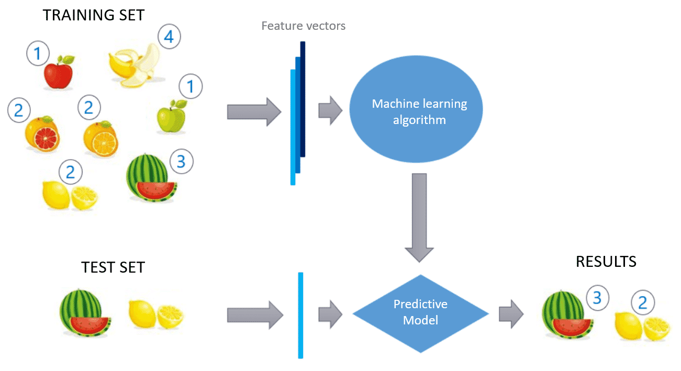
\includegraphics{./pic/chapter-0-0_pic_0.png}
\caption{chapter-0-0\_pic\_0.png}
\end{figure}

    A supervised learning task with discrete class labels, such as in the
previous example, is also called a \textbf{classification task}. Another
subcategory of supervised learning is regression, where the outcome
signal is a continuous value.

A second type of supervised learning is the prediction of continuous
outcomes, which is also called \textbf{regression analysis}. In
regression analysis, we are given a number of predictor (explanatory)
variables and a continuous response variable (outcome), and we try to
find a relationship between those variables that allows us to predict an
outcome. Note that in the field of machine learning, the predictor
variables are commonly called \textbf{\emph{features}}, and the response
variables are usually referred to as \textbf{\emph{target variables}}.

    \begin{figure}
\centering
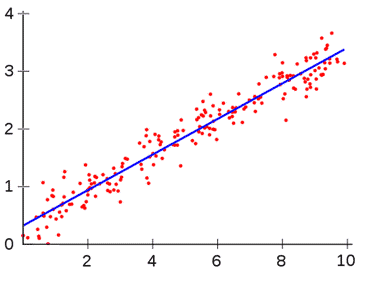
\includegraphics{./pic/chapter-0-0_pic_1.png}
\caption{chapter-0-0\_pic\_1.png}
\end{figure}

    \hypertarget{unsupervised-learning}{%
\subsubsection{Unsupervised Learning}\label{unsupervised-learning}}

    In supervised learning, we know the right answer beforehand when we
train a model. In \textbf{unsupervised learning}, however, we are
dealing with \textbf{\emph{unlabeled data}} or data of unknown
structure. Using unsupervised learning techniques, we are able to
explore the structure of our data to extract meaningful information
without the guidance of a known outcome variable or reward function.

\textbf{Clustering} is an exploratory data analysis technique that
allows us to organize a pile of information into meaningful subgroups
(clusters) \emph{without having any prior knowledge of their group
memberships}. Each cluster that arises during the analysis defines a
group of objects that share a certain degree of similarity but are more
dissimilar to objects in other clusters, which is why clustering is also
sometimes called unsupervised classification. Clustering is a great
technique for structuring information and deriving meaningful
relationships from data. For example, it allows marketers to discover
customer groups based on their interests, in order to develop distinct
marketing programs.

    \begin{figure}
\centering
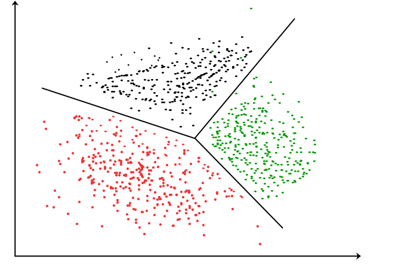
\includegraphics{./pic/chapter-0-0_pic_2.png}
\caption{chapter-0-0\_pic\_2.png}
\end{figure}

    \hypertarget{reinforcement-learning}{%
\subsubsection{Reinforcement Learning}\label{reinforcement-learning}}

    Another type of machine learning is \textbf{reinforcement learning}. In
reinforcement learning, the goal is to develop a system
(\textbf{\emph{agent}}) that improves its performance based on
interactions with the environment. Since the information about the
current state of the environment typically also includes a so-called
\textbf{reward signal}, we can think of reinforcement learning as a
field related to supervised learning. However, in reinforcement
learning, this feedback is not the correct ground truth label or value,
but a measure of how well the action was measured by a reward function.
Through its interaction with the environment, an agent can then use
reinforcement learning to learn a series of actions that maximizes this
reward via an exploratory trial-and-error approach or deliberative
planning. A popular example of reinforcement learning is a chess engine.
Here, the agent decides upon a series of moves depending on the state of
the board (the environment), and the reward can be defined as win or
lose at the end of the game.

    \hypertarget{features-and-labels}{%
\subsection{Features and Labels}\label{features-and-labels}}

The data for supervised learning contains whare are referred to as
\textbf{features} and \textbf{labels}. The \textbf{labels} are the
values of the target that is to be predicted. The \textbf{features} are
the variables from which the predictions are to be made. For example
when predicting the price of a house the \textbf{features} could be the
swuare meters of living space, the number of bedrooms, the number of
bathrooms, the size of the garage and so on. The \textbf{label} would be
the house price.

The data for unsupervised learning consists of features but no labels
because the model is being used to identify patterns not to forecast
something.

    \hypertarget{type-of-data}{%
\subsection{Type of Data}\label{type-of-data}}

There are two types of data:

\begin{itemize}
\tightlist
\item
  Numerical
\item
  Categorical
\end{itemize}

Numerical data consists of numbers. Categorical data is data which can
fall into a number of different categories, for example data to predict
a house price might categorize driveways as asphalt, concrete, grass,
etc. Categorical data must be converted to numbers for the purposes of
analysis.

The standard way of dealing with categorical features is to create a
dummy variable for each category. The value of this variable is 1 if the
feature is in the category and 0 otherwise. For example in the situation
in which individuals are categorized as male or female, we could create
two dummy variables. For man the first dummy variable would be 1 and the
second would be 0. The opposite for women. This procedure is appropriate
when there is no natural ordering between the feature values.

When there is a natural ordering, we can reflect this in the numbers
assigned. For example if the size of an order is classified as small,
medium or large, we can replace the feature by a numerical variable
where \emph{small = 1}, \emph{medium = 2} and \emph{large = 3}.

    \hypertarget{learning-tools}{%
\subsection{Learning Tools}\label{learning-tools}}

    \hypertarget{using-python-for-machine-learning}{%
\subsubsection{Using Python for machine
learning}\label{using-python-for-machine-learning}}

    Python is one of the most popular programming languages for data science
and thanks to its very active developer and open source community, a
large number of useful libraries for scientific computing and machine
learning have been developed. Although the performance of interpreted
languages, such as Python, for computation-intensive tasks is inferior
to lower-level programming languages, extension libraries such as
\textbf{NumPy}, \textbf{Matplotlib} and \textbf{Pandas}, among the
others, have been developed that build upon lower-layer Fortran and C
implementations for fast vectorized operations on multidimensional
arrays. For machine learning programming tasks, we will mostly refer to
the \textbf{scikit-learn} library, which is currently one of the most
popular and accessible open source machine learning libraries. In the
later chapters, when we focus on a subfield of machine learning called
deep learning, we will use the latest version of the \textbf{Keras}
library, which specializes in training so-called deep neural network
models very efficiently.

    \hypertarget{installing-python-and-packages}{%
\subsubsection{Installing Python and
Packages}\label{installing-python-and-packages}}

    To set up your python environment, you'll first need to have a python on
your machine. There are various python distributions available and we
have chosen one that works very well for data science:
\textbf{Anaconda}. Anaconda comes with its own Python distribution which
will be installed along with it.

Data Science often requires you to work with a lot of scientific
packages like scipy and numpy, data manipulation packages like pandas
and IDEs and interactive Jupyter Notebook.Now, you don't need to worry
about any python package most of them come pre-installed and if you want
to install a new package, you can do that simply by using conda or via
the pip installer program, which has been part of the Python Standard
Library since Python 3.3. More information about pip can be found
\href{https://docs.python.org/3/installing/index.html}{here}. After we
have successfully installed Python, we can execute pip from the terminal
to install additional Python packages:

\textbf{pip install SomePackage}

Already installed packages can be updated via the --upgrade flag:

\textbf{pip install SomePackage --upgrade}

To download an Anaconda distribution, you can use the
\href{https://www.anaconda.com/download/}{official download page} and
you can select your platform and then choose the installer. For this,
you can choose which version you want and whether 32-bit or 64-bit.

    \begin{figure}
\centering
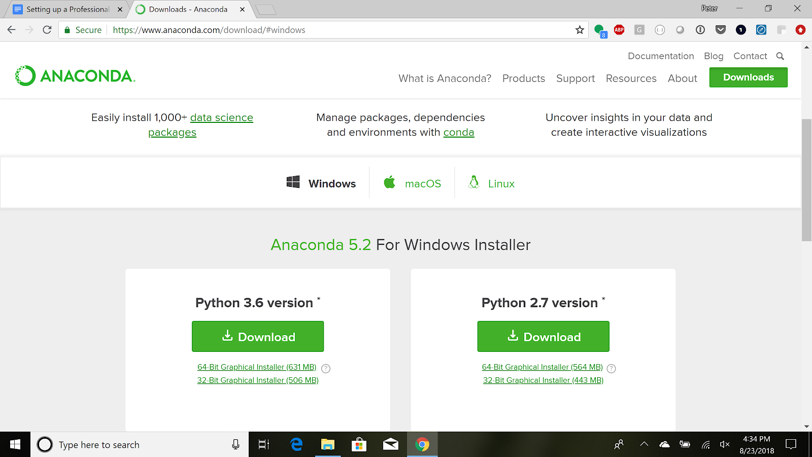
\includegraphics{./pic/chapter-0-0_pic_3.png}
\caption{chapter-0-0\_pic\_3.png}
\end{figure}

    To test your installation, on Windows, click on Start and then Anaconda
Navigator in the program list (or search for Anaconda in the search bar
and select Anaconda Navigator). On a Mac, open up the finder, and in the
Applications folder, double click on Anaconda-Navigator.

    \begin{figure}
\centering
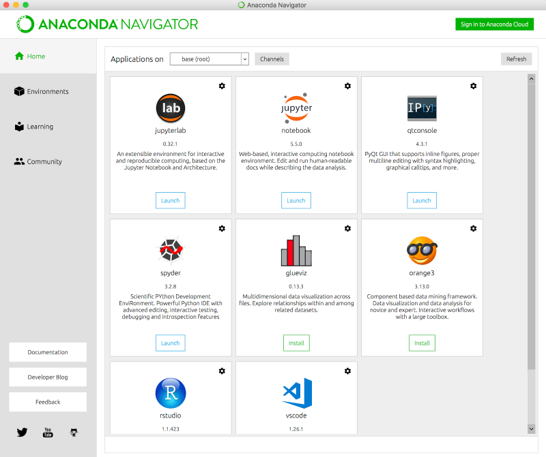
\includegraphics{./pic/chapter-0-0_pic_4.png}
\caption{chapter-0-0\_pic\_4.png}
\end{figure}

    \textbf{Package Managers}

Anaconda will give you two package managers- \textbf{pip} and
\textbf{conda}. When some packages aren't available with conda, you can
use pip to install them. Note that using pip to install packages also
available to conda may cause an installation error.

    \textbf{Jupyter Notebook}

A notebook is a document like this one! A notebook integrates code and
its output into a single document that combines visualizations,
narrative text, mathematical equations, and other rich media.

In other words: it's a single document where you can run code, display
the output, and also add explanations, formulas, charts, and make your
work more transparent, understandable, repeatable, and shareable. As
part of the open source Project Jupyter, Jupyter Notebooks are
completely free. You can download the software on its own, or as part of
the Anaconda data science toolkit.

    \textbf{Data Files}

\textbf{INSERIRE UNA DESCRIZIONE PRECISA DEI FILE DI DATI CHE VERRANNO
UTILIZZATI DOVE RECUPERARLI E DOVE TENERLI}

    \hypertarget{google-colab}{%
\subsubsection{Google Colab}\label{google-colab}}

    Although it is not essential to work in a colab environment (all the
course notebooks are in fact designed to be able to run without problems
locally on your pc), it is useful to know some basic elements of the
interaction with colab. In particular, in the cells below you will find
two examples for the use of external files. In the first case it is
shown how to load a text file from your local PC into the google virtual
machine. The second example relates to the opposite operation: let's
create a simple pandas dataframe into the colab environment and export
it in csv format to the local machine.

    \hypertarget{how-upload-a-file-on-google-colab}{%
\paragraph{How Upload a File on Google
Colab}\label{how-upload-a-file-on-google-colab}}

    \begin{tcolorbox}[breakable, size=fbox, boxrule=1pt, pad at break*=1mm,colback=cellbackground, colframe=cellborder]
\prompt{In}{incolor}{9}{\boxspacing}
\begin{Verbatim}[commandchars=\\\{\}]
\PY{k}{if} \PY{l+s+s1}{\PYZsq{}}\PY{l+s+s1}{google.colab}\PY{l+s+s1}{\PYZsq{}} \PY{o+ow}{in} \PY{n+nb}{str}\PY{p}{(}\PY{n}{get\PYZus{}ipython}\PY{p}{(}\PY{p}{)}\PY{p}{)}\PY{p}{:}
    \PY{k+kn}{from} \PY{n+nn}{google}\PY{n+nn}{.}\PY{n+nn}{colab} \PY{k+kn}{import} \PY{n}{files}
    \PY{n}{uploaded} \PY{o}{=} \PY{n}{files}\PY{o}{.}\PY{n}{upload}\PY{p}{(}\PY{p}{)}
    \PY{n}{path} \PY{o}{=} \PY{l+s+s1}{\PYZsq{}}\PY{l+s+s1}{\PYZsq{}}
\PY{k}{else}\PY{p}{:}
    \PY{n}{path} \PY{o}{=} \PY{l+s+s1}{\PYZsq{}}\PY{l+s+s1}{./data/}\PY{l+s+s1}{\PYZsq{}}
\end{Verbatim}
\end{tcolorbox}

    \begin{tcolorbox}[breakable, size=fbox, boxrule=1pt, pad at break*=1mm,colback=cellbackground, colframe=cellborder]
\prompt{In}{incolor}{10}{\boxspacing}
\begin{Verbatim}[commandchars=\\\{\}]
\PY{k}{with} \PY{n+nb}{open}\PY{p}{(}\PY{n}{path} \PY{o}{+} \PY{l+s+s2}{\PYZdq{}}\PY{l+s+s2}{carroll\PYZhy{}alice.txt}\PY{l+s+s2}{\PYZdq{}}\PY{p}{,} \PY{l+s+s2}{\PYZdq{}}\PY{l+s+s2}{r}\PY{l+s+s2}{\PYZdq{}}\PY{p}{)} \PY{k}{as} \PY{n}{f}\PY{p}{:}
    \PY{n}{alice} \PY{o}{=} \PY{n}{f}\PY{o}{.}\PY{n}{read}\PY{p}{(}\PY{p}{)}
    
\PY{n}{alice}\PY{p}{[}\PY{p}{:}\PY{l+m+mi}{392}\PY{p}{]}    
\end{Verbatim}
\end{tcolorbox}

            \begin{tcolorbox}[breakable, size=fbox, boxrule=.5pt, pad at break*=1mm, opacityfill=0]
\prompt{Out}{outcolor}{10}{\boxspacing}
\begin{Verbatim}[commandchars=\\\{\}]
"[Alice's Adventures in Wonderland by Lewis Carroll 1865]\textbackslash{}n\textbackslash{}nCHAPTER I. Down the
Rabbit-Hole\textbackslash{}n\textbackslash{}nAlice was beginning to get very tired of sitting by her sister on
the\textbackslash{}nbank, and of having nothing to do: once or twice she had peeped into
the\textbackslash{}nbook her sister was reading, but it had no pictures or conversations
in\textbackslash{}nit, 'and what is the use of a book,' thought Alice 'without pictures
or\textbackslash{}nconversation?'"
\end{Verbatim}
\end{tcolorbox}
        
    \hypertarget{how-download-a-file-on-google-colab}{%
\paragraph{How Download a File on Google
Colab}\label{how-download-a-file-on-google-colab}}

    \begin{tcolorbox}[breakable, size=fbox, boxrule=1pt, pad at break*=1mm,colback=cellbackground, colframe=cellborder]
\prompt{In}{incolor}{11}{\boxspacing}
\begin{Verbatim}[commandchars=\\\{\}]
\PY{k+kn}{import} \PY{n+nn}{pandas} \PY{k}{as} \PY{n+nn}{pd}

\PY{n}{cars} \PY{o}{=} \PY{p}{\PYZob{}}\PY{l+s+s1}{\PYZsq{}}\PY{l+s+s1}{Brand}\PY{l+s+s1}{\PYZsq{}}\PY{p}{:} \PY{p}{[}\PY{l+s+s1}{\PYZsq{}}\PY{l+s+s1}{Honda Civic}\PY{l+s+s1}{\PYZsq{}}\PY{p}{,}\PY{l+s+s1}{\PYZsq{}}\PY{l+s+s1}{Toyota Corolla}\PY{l+s+s1}{\PYZsq{}}\PY{p}{,}\PY{l+s+s1}{\PYZsq{}}\PY{l+s+s1}{Ford Focus}\PY{l+s+s1}{\PYZsq{}}\PY{p}{,}\PY{l+s+s1}{\PYZsq{}}\PY{l+s+s1}{Audi A4}\PY{l+s+s1}{\PYZsq{}}\PY{p}{]}\PY{p}{,}
        \PY{l+s+s1}{\PYZsq{}}\PY{l+s+s1}{Price}\PY{l+s+s1}{\PYZsq{}}\PY{p}{:} \PY{p}{[}\PY{l+m+mi}{22000}\PY{p}{,}\PY{l+m+mi}{25000}\PY{p}{,}\PY{l+m+mi}{27000}\PY{p}{,}\PY{l+m+mi}{35000}\PY{p}{]}
        \PY{p}{\PYZcb{}}

\PY{n}{df} \PY{o}{=} \PY{n}{pd}\PY{o}{.}\PY{n}{DataFrame}\PY{p}{(}\PY{n}{cars}\PY{p}{,} \PY{n}{columns}\PY{o}{=} \PY{p}{[}\PY{l+s+s1}{\PYZsq{}}\PY{l+s+s1}{Brand}\PY{l+s+s1}{\PYZsq{}}\PY{p}{,} \PY{l+s+s1}{\PYZsq{}}\PY{l+s+s1}{Price}\PY{l+s+s1}{\PYZsq{}}\PY{p}{]}\PY{p}{)}
\end{Verbatim}
\end{tcolorbox}

    \begin{tcolorbox}[breakable, size=fbox, boxrule=1pt, pad at break*=1mm,colback=cellbackground, colframe=cellborder]
\prompt{In}{incolor}{12}{\boxspacing}
\begin{Verbatim}[commandchars=\\\{\}]
\PY{k}{if} \PY{l+s+s1}{\PYZsq{}}\PY{l+s+s1}{google.colab}\PY{l+s+s1}{\PYZsq{}} \PY{o+ow}{in} \PY{n+nb}{str}\PY{p}{(}\PY{n}{get\PYZus{}ipython}\PY{p}{(}\PY{p}{)}\PY{p}{)}\PY{p}{:}
    \PY{c+c1}{\PYZsh{} if we run in google environment first we save in virtual machine...}
    \PY{n}{df}\PY{o}{.}\PY{n}{to\PYZus{}csv} \PY{p}{(}\PY{l+s+s1}{\PYZsq{}}\PY{l+s+s1}{export\PYZus{}dataframe.csv}\PY{l+s+s1}{\PYZsq{}}\PY{p}{,} \PY{n}{index} \PY{o}{=} \PY{k+kc}{False}\PY{p}{,} \PY{n}{header}\PY{o}{=}\PY{k+kc}{True}\PY{p}{)}
    \PY{c+c1}{\PYZsh{} ...then we download to local machine}
    \PY{k+kn}{from} \PY{n+nn}{google}\PY{n+nn}{.}\PY{n+nn}{colab} \PY{k+kn}{import} \PY{n}{files}
    \PY{n}{files}\PY{o}{.}\PY{n}{download}\PY{p}{(}\PY{l+s+s2}{\PYZdq{}}\PY{l+s+s2}{export\PYZus{}dataframe.csv}\PY{l+s+s2}{\PYZdq{}}\PY{p}{)}    
\PY{k}{else}\PY{p}{:}
    \PY{c+c1}{\PYZsh{} if we are working in local we save directly with the usual method}
    \PY{n}{df}\PY{o}{.}\PY{n}{to\PYZus{}csv} \PY{p}{(}\PY{l+s+s1}{\PYZsq{}}\PY{l+s+s1}{./data/export\PYZus{}dataframe.csv}\PY{l+s+s1}{\PYZsq{}}\PY{p}{,} \PY{n}{index} \PY{o}{=} \PY{k+kc}{False}\PY{p}{,} \PY{n}{header}\PY{o}{=}\PY{k+kc}{True}\PY{p}{)}
\end{Verbatim}
\end{tcolorbox}

    \hypertarget{packages-for-scientific-computing}{%
\subsection{Packages for scientific
computing}\label{packages-for-scientific-computing}}

Throughout this course, we will use \textbf{NumPy}'s multidimensional
arrays to store and manipulate data. We will make use of
\textbf{Pandas}, which is a library built on top of NumPy that provides
additional higher-level data manipulation tools that make working with
tabular data even more convenient. To augment your learning experience
and visualize quantitative data, which is often extremely useful to make
sense of it, we will use the very customizable \textbf{Matplotlib}
library.

    \hypertarget{summary}{%
\subsection{Summary}\label{summary}}

In this lesson, we explored machine learning at a very high level and
familiarized ourselves with the big picture and major concepts that we
are going to explore in the following chapters in more detail.

We learned that:

\begin{itemize}
\item
  \textbf{Supervised learning} is composed of two important subfields:
  \textbf{classification} and \textbf{regression}. While classification
  models allow us to categorize objects into known classes, we can use
  regression analysis to predict the continuous outcomes of target
  variables;
\item
  \textbf{Unsupervised learning} offers useful techniques for
  discovering structures in unlabeled data;
\item
  \textbf{How to set up a Python environment} and installed and updated
  the required packages to get ready to see machine learning in action.
\end{itemize}

    \hypertarget{textbooks-reference}{%
\subsection{Textbooks Reference}\label{textbooks-reference}}

These introductory lessons assume a basic level of statistical and
mathematical knowledge. No previous knowledge of Machine Learning is
assumed. For this reason I have decided to use \ldots{} basic texts for
the preparation of these lessons that you can consult for further
details on the topics we are going to deal with.

\begin{itemize}
\item
  John C. Hull, \textbf{Machine Learning in Business, An Introduction to
  the World of Data Science}, Amazon (2019)
\item
  Paul Wilmott\}, \textbf{Machine Learning, An Applied Mathematics
  Introduction}, Panda Ohana Publishing (2019)
\end{itemize}

    \hypertarget{appendix-a-machine-learning-terminology}{%
\subsection{Appendix A: Machine Learning
Terminology}\label{appendix-a-machine-learning-terminology}}

Machine learning is a vast field and also very interdisciplinary as it
brings together many scientists from other areas of research. As it
happens, many terms and concepts have been rediscovered or redefined and
may already be familiar to you but appear under different names. For
your convenience, in the following list, you can find a selection of
commonly used terms and their synonyms that you may find useful when
reading this book and machine learning literature in general:

\begin{itemize}
\item
  \textbf{Training example}: A row in a table representing the dataset
  and synonymous with an observation, record, instance, or sample (in
  most contexts, sample refers to a collection of training examples).
\item
  \textbf{Training}: Model fitting, for parametric models similar to
  parameter estimation.
\item
  \textbf{Feature}, abbrev. x: A column in a data table or data (design)
  matrix. Synonymous with predictor, variable, input, attribute, or
  covariate.
\item
  \textbf{Target}, abbrev. y: Synonymous with outcome, output, response
  variable, dependent variable, (class) label, and ground truth.
\item
  \textbf{Loss function}: Often used synonymously with a \textbf{cost
  function}. Sometimes the loss function is also called an error
  function. In some literature, the term ``loss'' refers to the loss
  measured for a single data point, and the cost is a measurement that
  computes the loss (average or summed) over the entire dataset.
\end{itemize}


    % Add a bibliography block to the postdoc
    
    
    
\end{document}
